\documentclass[prb,preprint]{revtex4-1} 
\raggedbottom
\usepackage{amsmath}
\usepackage{amsfonts}
\usepackage{graphicx}

\begin{document}

\section{Results and Analysis for Photon Counting}

We use a red laser (633 nm) which is attenuated by both a polarizer, lens, and a long metal tube. This laser is then directed towards a photomultiplier tube (PMT) which is used to amplify the laser signal to produce an output of discrete and well resolved pulses. Because the number of pulses is related to the intensity of light incident on the PMT we can, for constant intensity light, use counting statistics to determine the probability of counting $n$ photons in a time interval $T$. As such, we can write that probability, $P(n,T)$, as
\begin{equation}\label{const}
\binom{N}{n}=\frac{N!}{n!(N-n)!} \implies P(n,T)=\frac{(n_{\text{avg}})^{n}}{n!}\text{exp}(-n_{\text{avg}})
\end{equation}
for large $N$ and small $\delta t$, where $N$ is the number subdivisions in the time period $T$, and $N\delta t$=T. Additionally, on the right hand side of Eq \ref{const}, $n$ is the number of expected photons in $T$, while $n_\text{avg}$ is the measured average number of photons in $T$.

Furthermore we perform a similar analysis using a pseudo thermal source which is created by introducing a ground piece of glass whose purpose is to diffuses light. To account for this different source, which causes the intensity of light, $\lambda$, to vary, we use
\begin{equation}\label{pseudo}
P(n,T) = \frac{(\lambda_{\text{avg}}T)^n}{(\lambda_{\text{avg}}T+1)^{n+1}} = \frac{(n_{\text{avg}})^n}{(n_{\text{avg}}+1)^{n+1}}
\end{equation}
to describe the probability of counting $n$ photons in the time interval T, where $\lambda_\text{avg}$ is a measured average and is a term used to describe the probability that intensity of light is in really $\lambda$.

Using these theoretical equations we compare our measurements made with both the constant intensity light source and the pseudo thermal source. The following figures show the binned counts for the two sources at the average count rates of 1, 3, and 10 counts/ms. An ordinary $\chi^2$ squared test was also performed on each set of data and is listed in each figure's description.

\newpage

\begin{figure}[h]
\centering
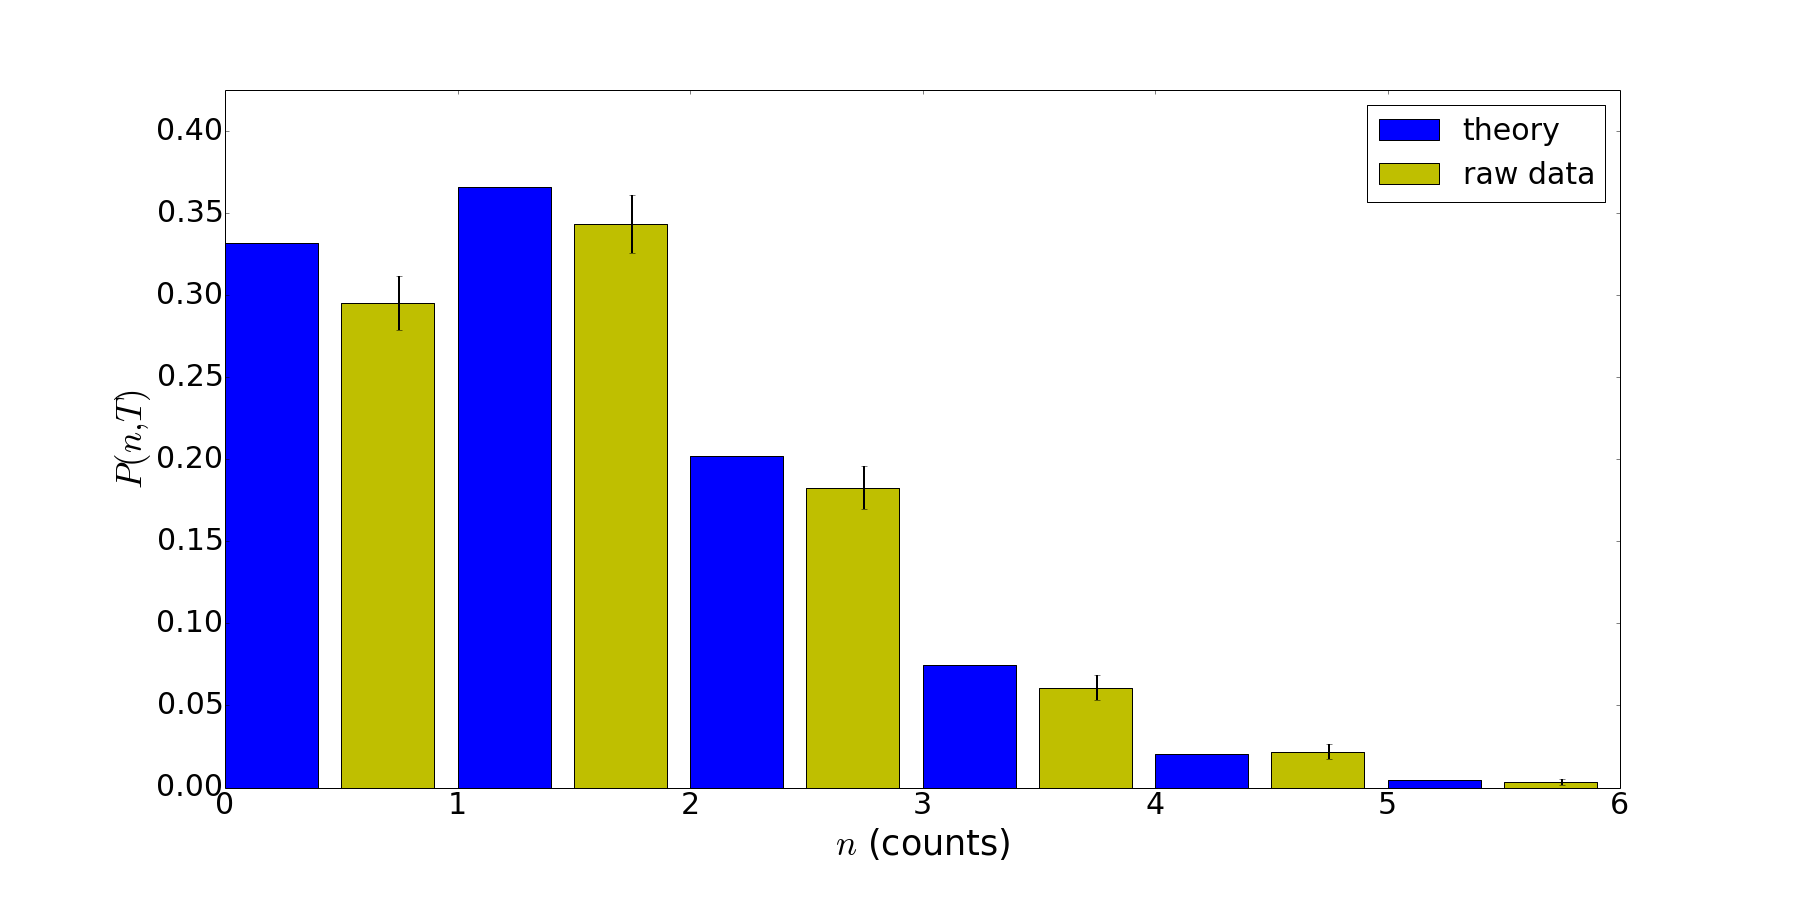
\includegraphics[width=0.9\textwidth]{1kc.png}
\caption{Shows the binned counts for a constant intensity source which averages approximately 1 counts per millisecond as compared to the theoretical distribution. $\chi^2$=1.757}
\label{LC2}
\end{figure}

\begin{figure}[h]
\centering
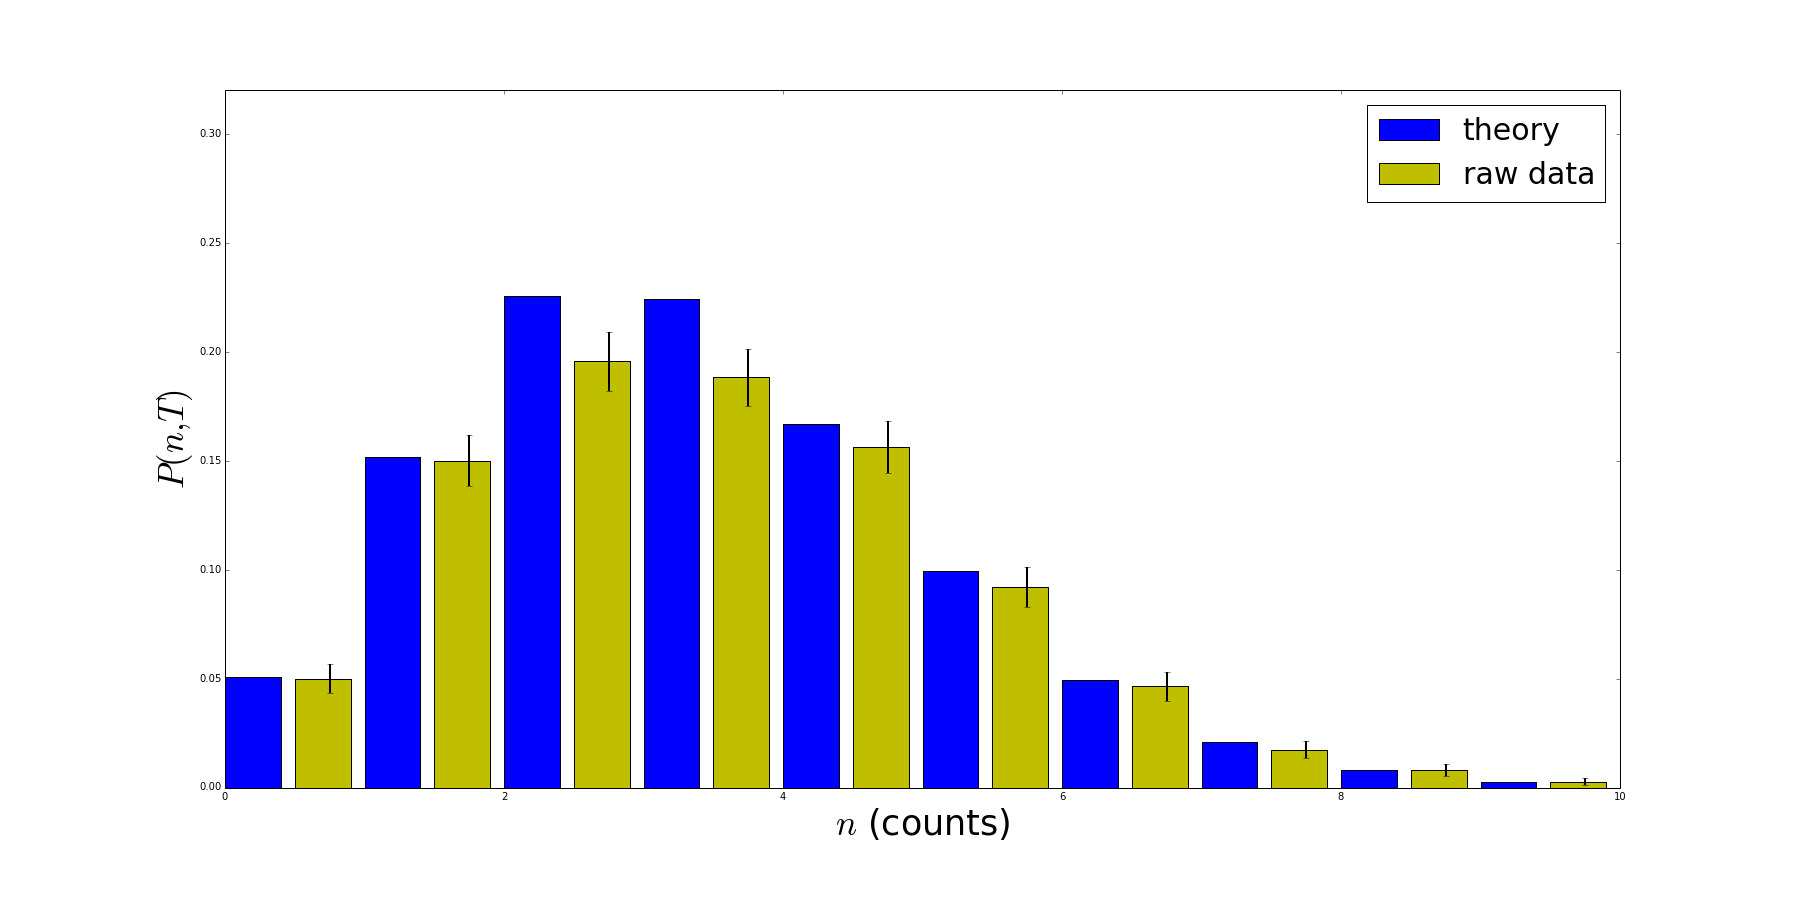
\includegraphics[width=0.9\textwidth]{3kc.png}
\caption{Shows the binned counts for a constant intensity source which averages approximately 3 counts per millisecond as compared to the theoretical distribution. $\chi^2$=1.525}
\label{LC2}
\end{figure}

\newpage

\begin{figure}[h]
\centering
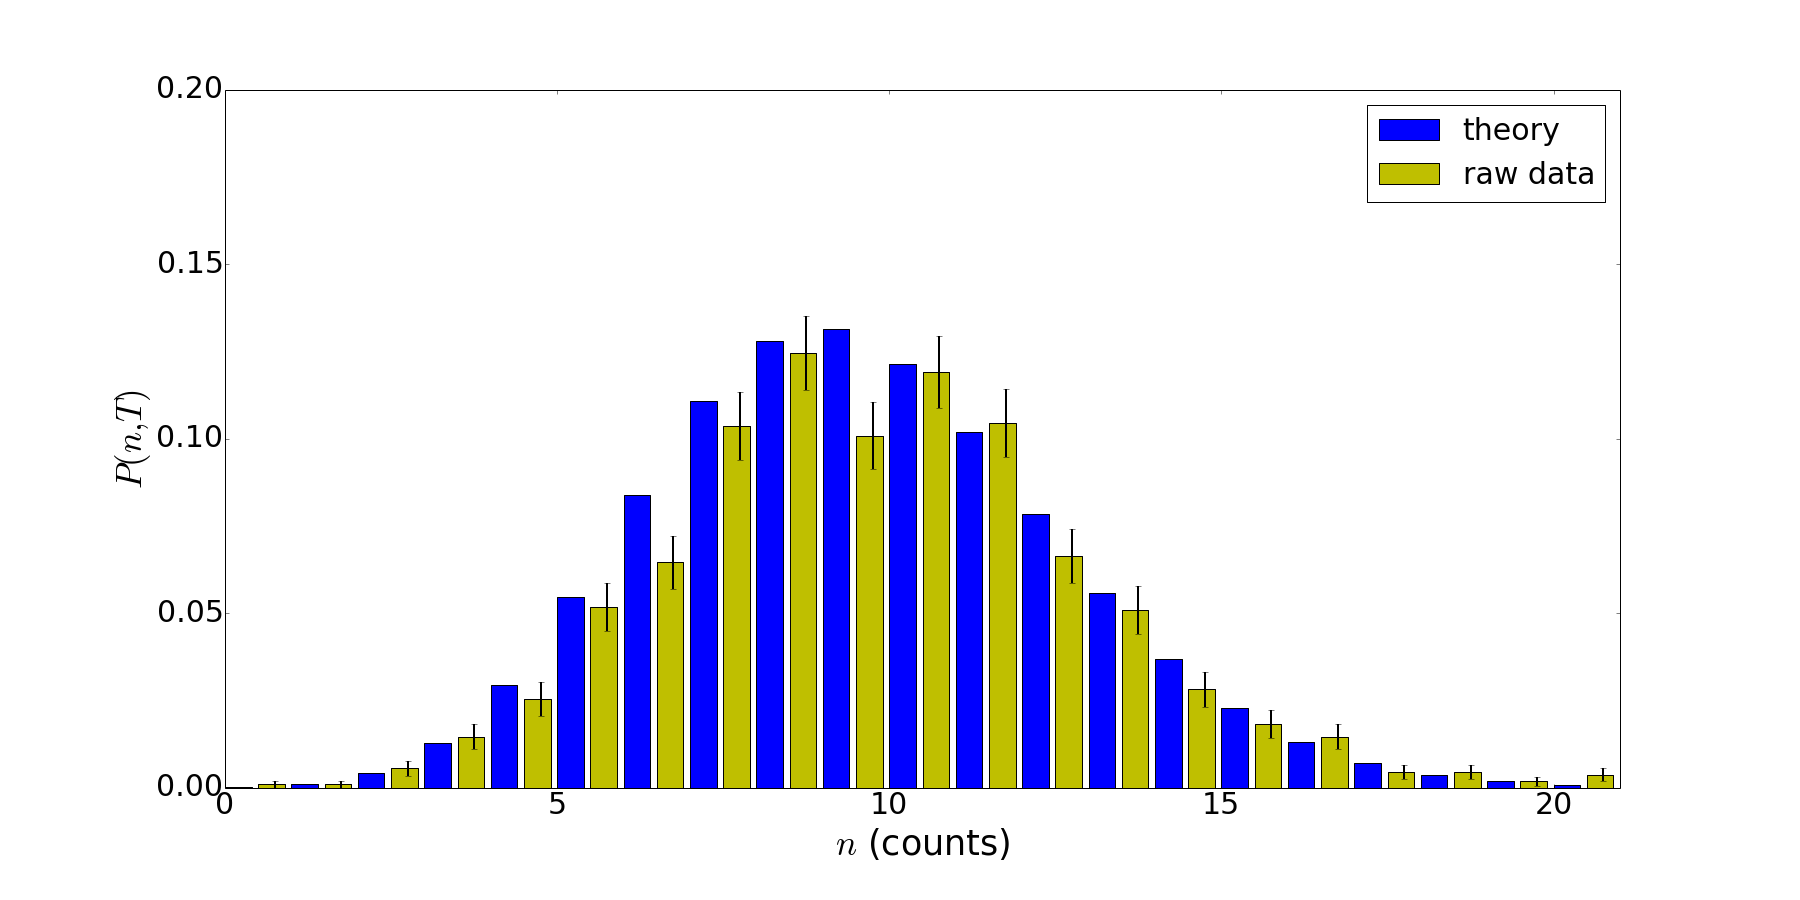
\includegraphics[width=0.9\textwidth]{10kc.png}
\caption{Shows the binned counts for a constant intensity source which averages approximately 10 counts per millisecond as compared to the theoretical distribution. $\chi^2$=1.473}
\label{LC2}
\end{figure}

\begin{figure}[h]
\centering
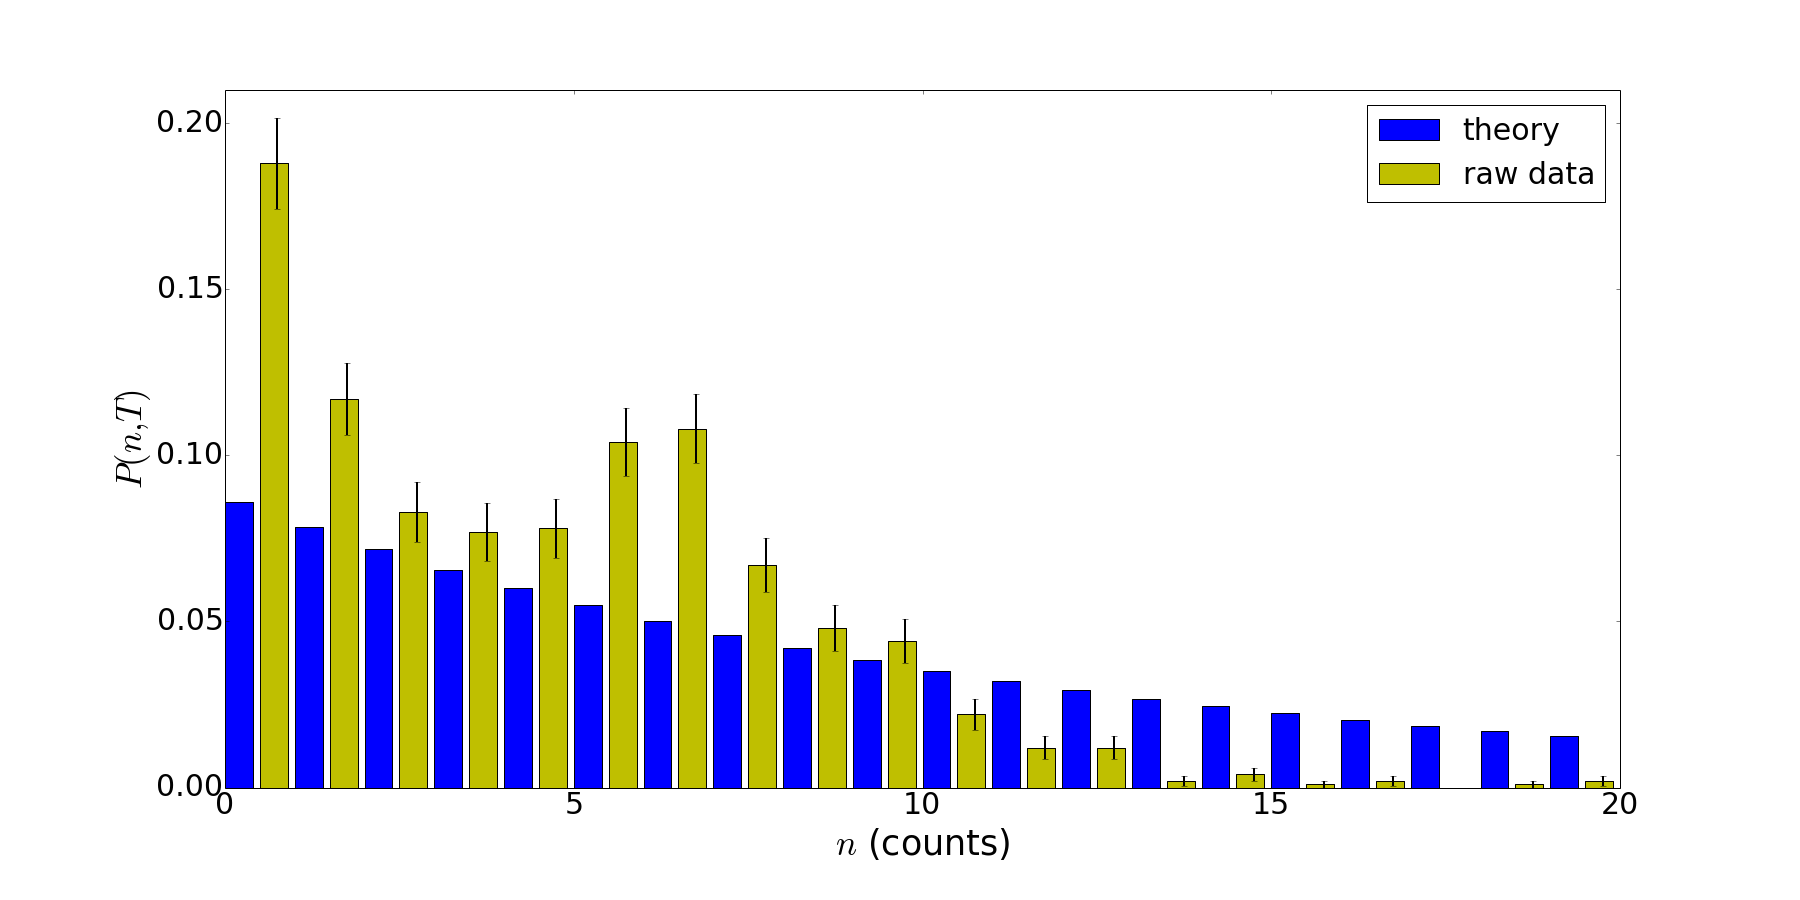
\includegraphics[width=0.9\textwidth]{1k.png}
\caption{Shows the binned counts for a variable intensity source which averages approximately 10 counts per millisecond as compared to the theoretical distribution. $\chi^2$=11.14}
\label{LC2}
\end{figure}

\newpage

\begin{figure}[h]
\centering
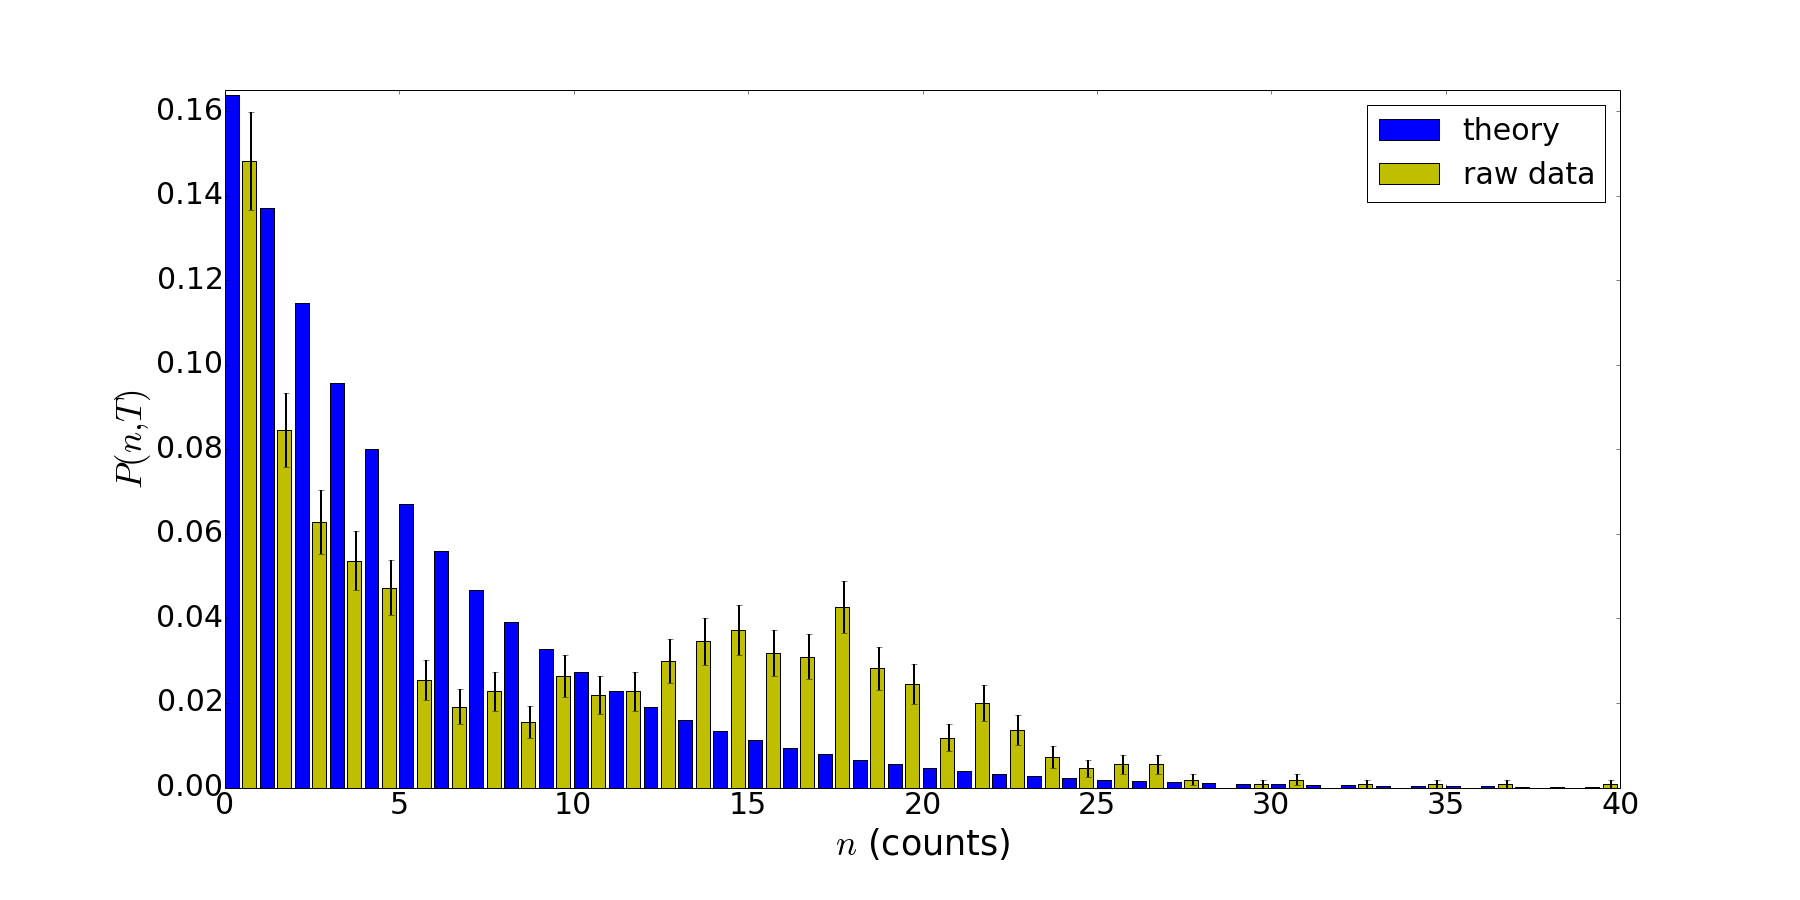
\includegraphics[width=0.9\textwidth]{3k.png}
\caption{Shows the binned counts for a variable intensity source which averages approximately 10 counts per millisecond as compared to the theoretical distribution. $\chi^2$=7.344}
\label{LC2}
\end{figure}

\begin{figure}[h]
\centering
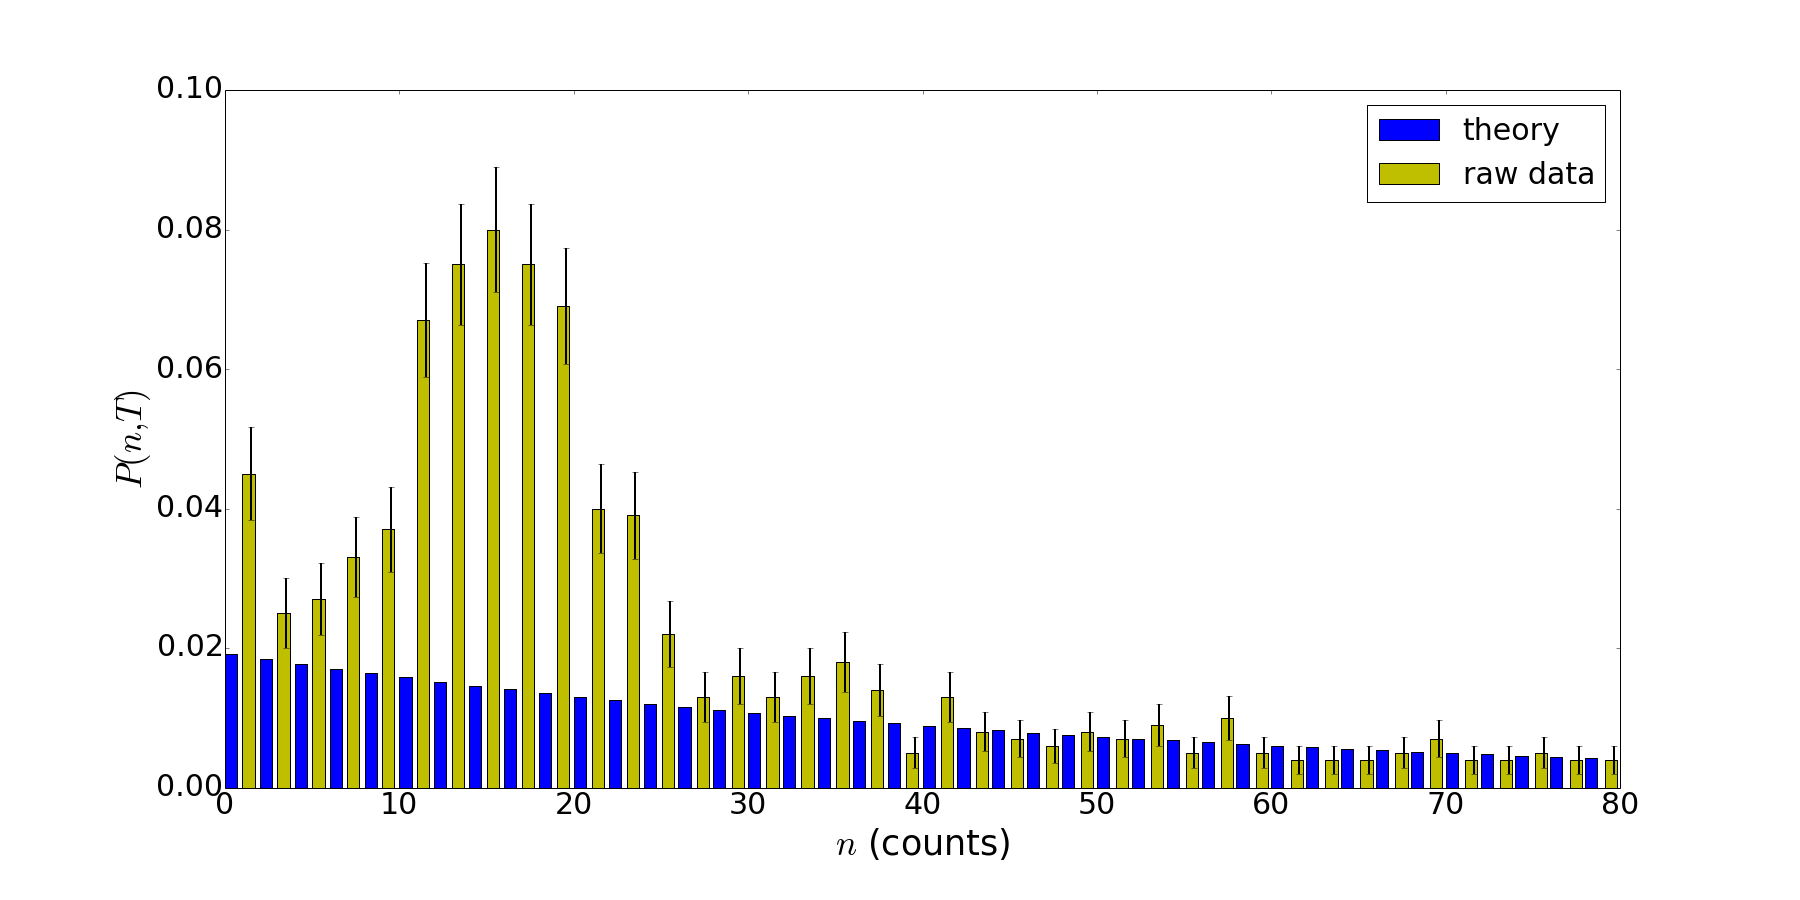
\includegraphics[width=0.9\textwidth]{10k.png}
\caption{Shows the binned counts for a variable intensity source which averages approximately 10 counts per millisecond as compared to the theoretical distribution. $\chi^2$=0.6323}
\label{LC2}
\end{figure}

\newpage

By analyzing the signal form the oscilloscope shown in Fig \ref{LC1} we can determine the gain for the PMT at our particular voltage input of 1 kV. To determine the number of electrons contained in the signal we examine the peak height and relate that to the current produced through the known internal resistance of 50 $\Omega$. Then by multiplying the current (charge/second) by the FWHM of the pulse which is measured in seconds we can identify the total charge in the pulse. Dividing charge in the pulse by the charge of a single electron then gives the number of electrons in the pulse. Using this method we find the gain of the PMT to be $\approx6\times10^7$ which compares nicely to the expected value from the maker of $\approx10^7$.

\begin{figure}[h]
\centering
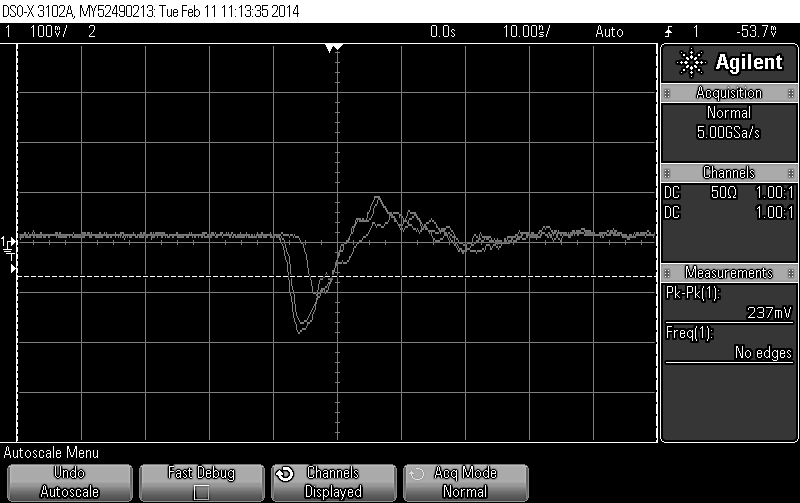
\includegraphics[width=0.75\textwidth]{scope_1.png}
\caption{A sample oscilloscope trace with an approximate FWHM of 8 ns which shows the pulse shape output by the PMT. Note the disturbance that follows the signal due to residual charge reaching the cathode following each detected photon.}
\label{LC1}
\end{figure}


\section{Conclusion}

Upon examination all data concerned with the pseudo thermal source contains unexpected peaks. The consistency in the kind of error suggests a systematic error. The nature of this error is unknown but may be due to an erroneous modal setting associated with the counter, or more likely the simple fact that the ground glass plate used to create speckle patterns was not a perfect thermal source.

\end{document}